% !TEX TS-program = pdflatex
% !TEX encoding = UTF-8 Unicode

% This is a simple template for a LaTeX document using the "article" class.
% See "book", "report", "letter" for other types of document.

\documentclass[11pt]{scrreprt} % use larger type; default would be 10pt

\usepackage[utf8]{inputenc} % set input encoding (not needed with XeLaTeX)
\usepackage{german}
%%% Examples of Article customizations
% These packages are optional, depending whether you want the features they provide.
% See the LaTeX Companion or other references for full information.

%%% PAGE DIMENSIONS
\usepackage{geometry} % to change the page dimensions
\geometry{a4paper} % or letterpaper (US) or a5paper or....
% \geometry{margins=2in} % for example, change the margins to 2 inches all round
% \geometry{landscape} % set up the page for landscape
%   read geometry.pdf for detailed page layout information

\usepackage{graphicx} % support the \includegraphics command and options

% \usepackage[parfill]{parskip} % Activate to begin paragraphs with an empty line rather than an indent

%%% PACKAGES
\usepackage{booktabs} % for much better looking tables
\usepackage{array} % for better arrays (eg matrices) in maths
\usepackage{paralist} % very flexible & customisable lists (eg. enumerate/itemize, etc.)
\usepackage{verbatim} % adds environment for commenting out blocks of text & for better verbatim
\usepackage{subfig} % make it possible to include more than one captioned figure/table in a single float
\usepackage{german}
\usepackage{url}
\usepackage[colorlinks=true]{hyperref}
\usepackage{amsfonts}
\usepackage{amsmath}
\usepackage{amsthm}
\usepackage{listings}
\usepackage{tikz}
\usepackage{pgfplots}
\usetikzlibrary{arrows,%
                petri,%
                topaths}%
\usepackage{tkz-berge}
\usepackage{algorithm}% http://ctan.org/pkg/algorithms
\usepackage{algpseudocode}% http://ctan.org/pkg/algorithmicx
% These packages are all incorporated in the memoir class to one degree or another...

\usepackage{listings}
\usepackage{color}
\definecolor{lightgray}{rgb}{.9,.9,.9}
\definecolor{darkgray}{rgb}{.4,.4,.4}
\definecolor{purple}{rgb}{0.65, 0.12, 0.82}

\lstdefinelanguage{JavaScript}{
  keywords={typeof, new, true, false, catch, function, return, null, catch, switch, var, if, in, while, do, else, case, break},
  keywordstyle=\color{blue}\bfseries,
  ndkeywords={class, export, boolean, throw, implements, import, this},
  ndkeywordstyle=\color{darkgray}\bfseries,
  identifierstyle=\color{black},
  sensitive=false,
  comment=[l]{//},
  morecomment=[s]{/*}{*/},
  commentstyle=\color{purple}\ttfamily,
  stringstyle=\color{red}\ttfamily,
  morestring=[b]',
  morestring=[b]"
}

\lstset{
   language=JavaScript,
   backgroundcolor=\color{lightgray},
   extendedchars=true,
   basicstyle=\footnotesize\ttfamily,
   showstringspaces=false,
   showspaces=false,
   %numbers=left,
   numberstyle=\footnotesize,
   numbersep=9pt,
   tabsize=2,
   breaklines=true,
   showtabs=false,
   captionpos=b
}

%%% HEADERS & FOOTERS
\usepackage{fancyhdr} % This should be set AFTER setting up the page geometry
\pagestyle{fancy} % options: empty , plain , fancy
\renewcommand{\headrulewidth}{0pt} % customise the layout...
\lhead{}\chead{}\rhead{}
\lfoot{}\cfoot{\thepage}\rfoot{}

%%% SECTION TITLE APPEARANCE
\usepackage{sectsty}
\allsectionsfont{\sffamily\mdseries\upshape} % (See the fntguide.pdf for font help)
% (This matches ConTeXt defaults)

%%% ToC (table of contents) APPEARANCE
\usepackage[nottoc,notlof,notlot]{tocbibind} % Put the bibliography in the ToC
\usepackage[titles,subfigure]{tocloft} % Alter the style of the Table of Contents
\renewcommand{\cftsecfont}{\rmfamily\mdseries\upshape}
\renewcommand{\cftsecpagefont}{\rmfamily\mdseries\upshape} % No bold!

%%% END Article customizations

%%% The "real" document content comes below...

\theoremstyle{definition}
\newtheorem*{beisp}{Beispiel}
\newtheorem{definition}{Definition}
\newtheorem*{bemerkung}{Bemerkung}

\title{Graph Coloring als Online-Problem mit bipartiten Graphen und Advice Complexity}
\subtitle{Semesterarbeit}
\author{Florian Lüthi\footnote{\url{luethifl@students.zhaw.ch}}}
\date{ZHAW, 22. November 2013} % Activate to display a given date or no date (if empty),
         % otherwise the current date is printed 

\begin{document}
\maketitle

\tableofcontents

\chapter{Einleitung}


\chapter{Advice Complexity}

\section{Online- vs. Offline-Probleme}

Optimierungsprobleme lassen sich (unter vielerlei anderen Klassifikationsmöglichkeiten) in Online-Probleme und Offline-Probleme mit dazugehörigen Online- bzw. Offline-Algo\-rithmen unterteilen. Der wesentliche Unterschied zwischen diesen beiden Klassen besteht darin, dass ein Offline-Algorithmus seine gesamte Eingabe zur Laufzeit kennt, während ein Online-Algorithmus dies nicht tut. Er bekommt einen Teil der Eingabe und berechnet daraus sofort einen Teil des Resultats. Ein solches Teilresultat kann im Nachhinein nicht mehr geändert werden.

Es liegt nun auf der Hand, dass ein Online-Algorithmus dazu tendiert, während der Berechnung eines Teilresultats Entscheidungen zu treffen, welche sich nach Berechnungen weiterer Teilresultate als suboptimal herausstellen -- dies insbesondere darum, weil die während der Berechnung des Teilresultats $i$ zur Verfügung stehenden Informationen über das gesamte Problem nur aus den Teileingaben der Berechnungen $1$ bis $i$ stammen können \cite{BKK}.

\bigskip
Eine weitere Folge des obengenannten Unterschieds manifestiert sich darin, dass ein Online-Algorithmus im Allgemeinen offensichtlich keine optimale Lösung findet. Auf der anderen Seite funktioniert ein qualitativer Vergleich zweier Algorithmen dadurch, dass deren asymptotische Laufzeitkomplexität verglichen wird. Da sich die Qualität der von einem Online-Algorithmus und dessen Offline-Pendant produzierten Lösungen grundlegend unterscheidet (während letzterer eine optimale Lösung anstrebt, ist ersterem diese konzeptbedingt verwehrt), muss eine andere Möglichkeit gefunden werden, diese beiden Algorithmen (und deren Lösungen) vergleichen zu können.

\section{Competitive Ratio}

Eine gängige Möglichkeit, dieses Problem zu lösen, ist die von Sleator und Tarjan eingeführte {\it Competitive Ratio} \cite{Sleator, BKK}, welche im Grunde genommen das Verhältnis zwischen den Kosten der optimalen Lösung und derer des zu untersuchenden Online-Algorithmus ausdrückt \cite{BKK}. Da die Qualität der Lösung eines Online-Algorithmus wesentlich von der Beschaffenheit der Eingabe abhängt, wird dabei vom jeweils schlechtestmöglichen Fall ausgegangen \cite{Trevisan}.

\bigskip
Formal kann die Competitive Ratio folgendermassen definiert werden: Sei $\operatorname{opt}(I)$ die optimale Lösung eines konkreten Online-Problems für eine Sequenz aus Teileingaben $I$. $\mathcal{I}$ sei die Menge aller möglicher solcher Sequenzen. Seien ferner $\mathcal{S}$ alle möglichen Lösungen (mit $\operatorname{opt}(I) \in \mathcal{S}$), $A(I) \in \mathcal{S}$ diejenige Lösung, welche der Online-Algorithmus zu diesem Problem liefern kann, und $C : \mathcal{S} \rightarrow \mathbb{R}$ die Kosten für die jeweilige Lösung.

\bigskip
Ein Online-Algorithmus wird nun als {\it $c$-kompetitiv} bezeichnet, wenn es Konstanten $c \ge 0$ und $\alpha$ gibt, sodass für sämtliche mögliche Eingaben $I$
\[
C(A(I)) \le c\cdot C(\operatorname{opt}(I)) + \alpha
\]
gilt \cite{BKK}, und die Competitive Ratio wäre ergo
\[
c = \max_{I \in \mathcal{I}} \left\{ \frac {C(A(I))}{C(\operatorname{opt}(I))} \right\}.
\]

\section{Das {\sc SkiRental}-Problem}

Die Competitive Ratio lässt sich durch das wohlbekannte {\sc SkiRental}-Problem illustrieren: Nehmen wir an, wir wollen zum ersten Mal ein Wochenende lang Skifahren gehen. Wir besitzen aber keine Skis. Es stellt sich nun die Frage, ob wir Skis mieten oder kaufen wollen -- wobei erschwerend hinzukommt, dass wir momentan noch keine Ahnung haben, wieviele Wochenenden wir danach noch skifahrend verbringen möchten.

Angenommen, der Kauf eines Paars Ski kostet CHF 500, die Miete äquivalenter Skis für ein Wochenende hingegen CHF 50.\footnote{In der Realität wesentliche Aspekte wie Preisveränderungen über die Zeit, veränderte Qualitätsansprüche und Abnützung der Skis sollen bei dieser Betrachtung vernachlässigt werden.} Es ist nun einfach auszurechnen, dass sich der Kauf der Skis vor dem ersten Wochenende nur lohnen würde, wenn wir an mindestens 10 Wochenenden Skifahren gehen würden.

\bigskip
Da wir das aber nicht wissen, sind wir quasi der Online-Algorithmus, der für jede Teileingabe (sprich für jedes geplante Skiwochenende) sofort die Frage nach Kauf oder Miete beantworten muss. Die Teileingabe für den Algorithmus ist jeweils die Anzahl an vergangenen Skiwochenenden.

Die oben besprochene Eigenschaft der potenziellen Suboptimalität der Entscheidungen wird beim zehnten solchen Wochenende augenscheinlich, wenn bei den vorangegangen Wochenenden die Entscheidung jeweils auf Mieten gefallen sein sollte.

\bigskip
Bezeichne $t$ nun dasjenige Wochenende, an welchem wir uns dafür entscheiden, die Skis zu kaufen. Wir schauen uns die folgenden Fälle an:

\begin{itemize}
\item Für $t = 1$ gilt, dass $A(I) = 500$, denn wir kaufen ja gleich beim ersten Mal. Die Competitive Ratio $c$ hingegen liegt bei $10$, da wir im schlechtesten Fall nur dieses eine Mal Skifahren gehen -- es gälte also $\operatorname{opt}(I) = 50$.

\item Für $t = 2$ gilt, dass $A(I) = 550$, denn wir mieten beim ersten (CHF 50) und kaufen beim zweiten Mal (CHF 500). Die Competitive Ratio $c$ liegt bei $5.5$, da wir im schlechtesten Fall nur diese zwei Male Skifahren gehen -- optimal wäre zwei Mal mieten, also  $\operatorname{opt}(I) = 50$.

\item Für $t = 10$ gilt, dass $A(I) = 950$, denn wir mieten die ersten neun Male (CHF 450) und kaufen beim zehnten Mal (CHF 500). Für die optimale Lösung spielt es keine Rolle, ob gemietet oder gekauft wird, also ist $\operatorname{opt}(I) = 500$. Dies ergibt eine Competitive Ratio von $c = 1.9$.

\item Für $t = 11$ gilt, dass $A(I) = 1000$, denn wir mieten die ersten zehn Male (CHF 500) und kaufen beim elften Mal (CHF 500). Die Competitive Ratio $c$ liegt bei $c = 2$, da es optimal wäre, gleich beim ersten Mal die Skis zu kaufen (CHF 500).
\end{itemize}

Der Verlauf von $\operatorname{opt}(I)$ und $A(I)$ ist in Abbildung \ref{fig.skirental} skizziert, Abbildung \ref{fig.skirental.c} zeigt $c$ in Abhängigkeit von $t$.

\begin{figure}
\caption{Verlauf von Lösung und Optimum für SkiRental}
\label{fig.skirental}
\begin{center}
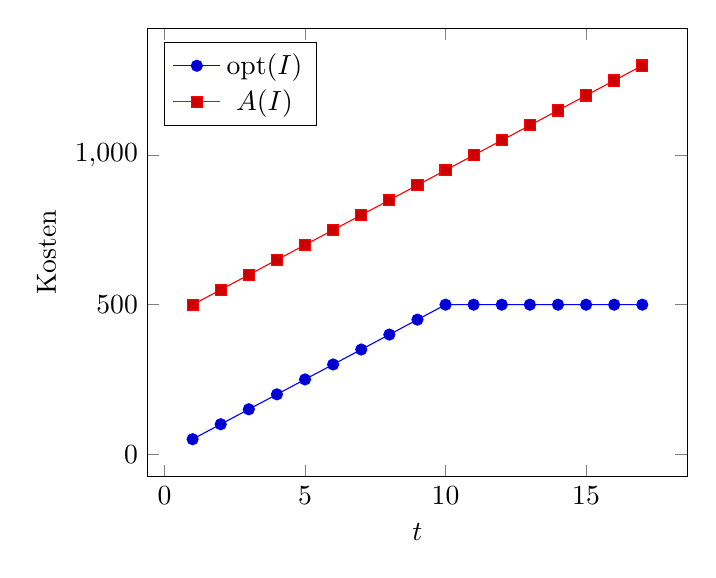
\begin{tikzpicture}
  \begin{axis}[ 
    xlabel=$t$,
    ylabel={Kosten},
	legend pos=north west
  ] 
    \addplot coordinates {
		(1,50)
		(2,100)
		(3,150)
		(4,200)
		(5,250)
		(6,300)
		(7,350)
		(8,400)
		(9,450)
		(10,500)
		(11,500)
		(12,500)
		(13,500)
		(14,500)
		(15,500)
		(16,500)
		(17,500)
	};
	\addlegendentry{$\operatorname{opt}(I)$}
    \addplot coordinates {
		(1,500)
		(2,550)
		(3,600)
		(4,650)
		(5,700)
		(6,750)
		(7,800)
		(8,850)
		(9,900)
		(10,950)
		(11,1000)
		(12,1050)
		(13,1100)
		(14,1150)
		(15,1200)
		(16,1250)
		(17,1300)
	};
	\addlegendentry{$A(I)$}
  \end{axis}
\end{tikzpicture}
\end{center}
\end{figure}

\begin{figure}
\caption{Verlauf der Competitive Ratio für SkiRental}
\label{fig.skirental.c}
\begin{center}
\begin{tikzpicture}
  \begin{axis}[ 
    xlabel=$t$,
    ylabel={$c(t)$},
	legend pos=north west
  ] 
    \addplot coordinates {
		(1,10)
		(2,5.5)
		(3,4)
		(4,3.25)
		(5,2.8)
		(6,2.5)
		(7,2.2857142857)
		(8,2.125)
		(9,2)
		(10,1.9)
		(11,2)
		(12,2.1)
		(13,2.2)
		(14,2.3)
		(15,2.4)
		(16,2.5)
		(17,2.6)
	};
  \end{axis}
\end{tikzpicture}
\end{center}
\end{figure}

\bigskip
Allgemein kann die Competitive Ratio für dieses Problem (mit allgemeinen Kosten $b$ für den Kauf bzw. $r$ für die Miete) beschrieben werden als
\[
	c(t) = \begin{cases}
		\frac{b+(t-1)\cdot r}{t\cdot r}, & \text{wenn } r\cdot t \le b \\
		\frac{b+(t-1)\cdot r}{b}, & \text{sonst}.
	\end{cases}
\]

Unsere Instanz des {\sc SkiRental}-Problems ist also $1.9$-kompetitiv; im Allgemeinen ist {\sc SkiRental} $(2-\frac r b)$-kompetitiv \cite{Dobrev}.

\bigskip
Zurück auf die Realität bezogen, scheint es eine sinnvolle Strategie bei {\sl Kaufen oder Mieten}-Problemen zu sein, das Objekt zu dem Zeitpunkt zu kaufen, an dem die kumulierten Mietkosten die Kaufkosten aufwiegen oder überschreiten -- die Competitive Ratio ist zu diesem Zeitpunkt die beste. Ausserdem kann die Annahme getroffen werden, dass die Wahrscheinlichkeit für eine weitere Benutzung des entsprechenden Objekts um einen mindestens gleich langen Zeitraum wie während der Mietphase (während welcher sich die Kaufkosten amortisieren) relevant ist \cite{Trevisan}.


\section{Das Orakel}

Es ist augenscheinlich, dass die Lösung $t = 10$ für unsere Instanz des {\sc SkiRental}-Problems die beste Approximation ist, welche wir erreichen können, solange wir nicht in die Zukunft schauen können. Nichtsdestotrotz ist diese Lösung offensichtlich weit entfernt davon, optimal zu sein -- im schlechtesten Fall würden wir $1.9$ mal so viel für unsere Skis bezahlen wie eigentlich nötig.

\bigskip
Entsprechend interessant wäre es, eine Aussage darüber machen zu können, wieviel zusätzliche Information der Online-Algorithmus zur Verfügung haben müsste, um das Problem optimal (oder mit einer festgelegten Competitive Ratio \cite{BKK}) lösen zu können. Während die Competitive Ratio die Kosten darstellt, welche durch die gefundene Lösung zusätzlich zur optimalen Lösung zu gewärtigen wären, würde diese Aussage den Zusatznutzen beschreiben, welcher sich durch den Preis dieser zusätzlichen Kosten erkaufen liesse \cite{Dobrev}.

\bigskip
Für unser {\sc SkiRental}-Problem ist die Antwort denkbar trivial: Es ist vollkommen ausreichend, bei der ersten Entscheidung (sprich bei der Berechnung des ersten Teilresultats) zu wissen, ob die Skis gekauft werden  oder ob sie für dieses und alle weiteren Wochenenden gemietet werden sollen -- mit einem einzigen Bit zusätzlicher Information könnte das Problem also optimal gelöst werden.

\bigskip
{\sc SkiRental} ist insofern speziell, als dass dem ganzen Leben (und damit auch der Freizeitplanung) nichtdeterministische Aspekte innewohnen; aus diesem Grunde wird die benötigte Information von keiner Instanz geliefert werden können. Auf der anderen Seite sind aber durchaus Probleme denkbar, welche eigentlich Online-Probleme sind (oder aus praktischen Gründen von Online-Algorithmen gelöst werden), die Qualität der Resultat aber nachhaltig verbessert werden könnte, wenn zusätzliche Offline-Informationen aus der gesamten Eingabe herangezogen werden könnten. Deren Beschaffung könnte mit derart hohen Kosten verbunden sein, dass die Bestrebung wäre, einen möglichst guten Kompromiss zwischen diesen Kosten und der verbesserten Competitive Ratio zu erreichen \cite{Dobrev}.

\bigskip
Interesssant wäre es darum, ein Modell zur Verfügung zu haben, mit welchem sich Probleme nach Anzahl und Art der zusätzlich benötigten Informationen klassifizieren liessen. \cite{Dobrev} schlägt ein solches Modell vor \cite{BKK} -- die sogenannte {\sl Advice Complexity}. Das Modell nimmt die Existenz eines {\sl Orakels} $\mathcal{O}$ an, welchem das Problem in seiner Gesamtheit bekannt ist und welches über unlimitierte Rechenleistung verfügt \cite{Dobrev, BKK}. Das Orakel stellt dem Algorithmus $\mathcal{A}$ bitweise Informationen zur Verfügung \cite{Dobrev}. Das Mass der {\sl Advice Complexity} bezeichnet demzufolge die Menge der zwischen dem Algorithmus und dem Orakel ausgetauschten Informationen. Da diese Menge an Informationen generell von der Länge der Eingabe abhängt, bezeichnet die Advice Complexity von $\mathcal{A}$ für Eingaben der Länge $n$ das Maximum an Advice Complexitiy für alle Abfragen für Totaleingaben mit maximaler Länge von $n$, normalisiert auf $n$ \cite{BKK}:

\[
	B_{(\mathcal{A}, \mathcal{O})} = \max_{I \in \mathcal{I}^n} \frac { B_{(\mathcal{A}, \mathcal{O})}(I) }{n},
\]

während die Advice Complexity des Problems $\mathcal{P}$ definiert ist als diejenige Advice Complexity des besten Algorithmus \cite{bipartite}.

\bigskip

\cite{Dobrev} schlägt vor, die Kommunikation zwischen dem Orakel und dem Algorithmus in wahlweise zwei verschiedenen Modi ablaufen zu lassen:

\begin{itemize}
\item Im {\sl Answerer}-Modus entscheidet der Algorithmus selbständig, ob und für welche Eingaben er das Orakel um Rat fragen muss. Für jede Anfrage schickt das Orakel einen Advice-String zurück, welcher aber nicht leer sein kann \cite{Dobrev} (denn dies wäre ja kein sinnvoller Rat).

Bezogen auf {\sc SkiRental} würde der Algorithmus das Orakel vor dem ersten Wochenende fragen, ob er die Skis kaufen oder mieten soll, und das Orakel würde diese Frage mit {\sl Kaufen} oder {\sl Mieten} beantworten. Danach wäre keine weitere Kommunikation zwischen Orakel und Algorithmus notwendig.

\item Im {\sl Helper}-Modus schickt das Orakel dem Algorithmus sporadisch und spontan Advices. Wir können uns das so vorstellen, dass der Algorithmus mehrere voneinander unabhängige Verhaltensmuster für die Berechnung der Teilausgabe aufweist, welche vom Orakel entsprechend aufgerufen werden können. Bei jedem notwendigen Wechsel des Verhaltensmusters würde das Orakel erneut einen Advice senden.

Bezogen auf {\sc SkiRental} würde das Orakel den Algorithmus vor dem ersten Wochenende entweder in den {\sl Kaufen}- oder {\sl Mieten}-Modus versetzen. Der {\sl Kaufen}-Modus kauft die Skis für die erste Teileingabe und tut nichts mehr für alle folgenden Teileingaben, während der {\sl Mieten}-Modus für jede Teileingabe die Skis mietet.
\end{itemize}

\bigskip

Wir beobachten, dass die Länge der vom Orakel gegebenen Advice-Strings ebenfalls Informationen beinhalten (beispielsweise zeigt ein leerer String im {\sl Helper}-Modus dem Algorithmus an, das momentane Verhaltensmuster beizubehalten). Dies ist insofern ein Problem, als dass es das Modell einerseits komplexer als notwendig macht. Andererseits wird der Vergleich von Advice Complexity mit anderen Komplexitätsmassen dadurch erschwert \cite{BKK}.

\cite{BKKR} entwickelt dieses Modell der Advice Complexity dahingehend weiter, als dass die Existenz eines {\sl Advice Tapes} angenommen wird, wohin das Orakel alle Advices sequentiell schreibt, und zwar vor der Berechnung der ersten Teileingabe durch den Algorithmus. Dadurch wird das Modell direkt vergleichbar mit demjenigen von randomisierten Online-Algorithmen \cite{BKK}; es kann konstatiert werden, dass für jeden randomisierten Online-Algorithmus $\mathcal{R}$, welcher $b$ Bits von seinem Random-Tape liest und eine Competitive Ratio von $r$ erreicht, ein Algorithmus mit Advice $\mathcal{A}$ und Orakel $\mathcal{O}$ existiert, welcher $b$ Advice-Bits benötigt und dessen Competitive Ratio ebenfalls $r$ ist \cite{BKKR}. Dies ist einfach durch die Konstruktion von $\mathcal{O}$ dahingehend zu erreichen, dass $\mathcal{O}$ dieselben Bits auf das Advice Tape schreibt, wie auf dem Random Tape für den randomisierten Algorithmus stehen würden.

\section{Online {\sc SimpleKnapsack} mit Advice}

Um die teilweise überraschenden Fähigkeiten von Algorithmen mit Advice zu demonstrieren, wollen wir uns das {\sc SimpleKnapsack}-Problem anschauen: Wir nehmen die Existenz eines Rucksacks an. Dieser Rucksack hat eine maximale Kapazität von $1$. Des weiteren nehmen wir eine Menge von Gegenständen $S = \{ w_1, \dots, w_n \}$ (deren $w_i$ die entsprechenden Grössen ausdrücken, mit $0 < w_i \le 1$) an. Das Ziel ist, den Rucksack möglichst gut (aber nur bis zur Kapazitätsgrenze) zu füllen.

Erschwerend kommt noch hinzu, dass dieses Problem als Online-Problem formuliert wird -- der Algorithmus bekommt also einen Gegenstand präsentiert und muss sofort entscheiden, ob er diesen im Rucksack verstauen will oder nicht. Das nachträgliche Entfernen von bereits verstauten Gegenständen ist nicht erlaubt \cite{knapsack}.

\bigskip
Allgemein existiert kein kompetitiver deterministischer Online-Algorithmus \cite{spaccamela}; die einzige Möglichkeit besteht im Grunde genommen darin, sämtliche präsentierten Gegenstände der Reihe nach einzupacken, solange sie noch in den Rucksack passen. Ein möglicher Adversary wäre nun die Sequenz $\langle \varepsilon, 1 \rangle$, wobei $\varepsilon$ beliebig nahe an $0$ gewählt werden könnte; dies führt dazu, dass der Algorithmus $\varepsilon$ in den Rucksack packt und dann aufhören muss, weil $\varepsilon + 1$ die Kapazitätsgrenze überschreiten würde.

Die Competitive Ratio dieses Algorithmus wäre entsprechend
\[
	r = \lim_{\varepsilon \rightarrow 0} \frac {1} { \varepsilon} = \infty.
\]

Wenn wir nun ein Orakel dazudenken, welches dem Algorithmus bei der ersten Entscheidung mitteilt, ob in der Sequenz ein Gegenstand $w_i$ vorkommt, für welchen $w_i \ge 0.5$ gilt, könnte der Algorithmus folgende Fallunterscheidung machen:

\begin{enumerate}[a)]
\item Falls ein solcher Gegenstand vorkommt, würde der Algorithmus solange alle Gegenstände verwerfen, bis ein Gegenstand mit $w_i \ge 0.5$ zur Debatte steht. Diesen würde er wie auch alle nachfolgenden in den Rucksack packen. Da er zumindest ersteren gepackt hat, hätte der Rucksack mindestens eine Gesamtfüllung von $0.5$.
\item Falls hingegen kein solcher Gegenstand vorkommt, würde der Algorithmus von Anfang an alle Gegenstände in den Rucksack packen. Der Rucksack wäre damit ebenfalls zu mindestens zur Hälfte gefüllt, da es keinen Gegenstand $\ge 0.5$ geben kann, der nicht in den Rucksack passen würde (ansonsten Fall a) zur Anwendung gelangt wäre).
\end{enumerate}

Daraus folgt, dass die Competitive Ratio des Algorithmus mit einem einzigen Advice Bit
\[
	r = \frac 1 {0.5} = 2
\]
ist \cite{knapsack}.

\bigskip
Spannenderweise wird die Competitive Ratio für $b \in \mathcal{O}(1)$ nicht wesentlich verbessert. Der Grund dafür ist im Prinzip, dass eine konstante Anzahl an Advice Bits nicht ausreichen kann, um genügend Informationen darüber transportieren zu können, welche Gegenstände ausgewählt werden sollen. Für $b \in \mathcal{O}(\log(n))$ gilt dies hingegen -- die Competitive Ratio reduziert sich dann auf $r = 1 + \varepsilon$ \cite{knapsack}.









\chapter{Online Graph Coloring von bipartiten Graphen}

\section{Modelle von (bipartiten) Graphen}

Im weiteren Verlauf dieser Arbeit wollen wir uns mit einer speziellen Variante des Graphenfärbeproblems beschäftigen. Damit wir dies tun können, wollen wir einige Begriffe definieren:

\begin{definition}[Graph]

Ein (ungerichteter, ungewichteter) Graph ist ein Tupel
\[
	G = (V, E),
\]
wobei $V = \{v_1, v_2, \dots \}$ dessen Knoten {\sl (vertices)} bezeichnet und $E = \{ e_1, e_2 \}$ dessen Kanten {\sl (edges)}. Jedes $e$ ist eine 2-elementige Teilmenge von $V$. \cite{biggs}

\end{definition}

Abbildung \ref{graph} illustriert einen Graphen mit
\[
	V = \{v_1,v_2,v_3,v_4,v_5,v_6\}
\]
und
\[
	E = \left\{  \{v_1,v_2\}, \{v_3,v_6\}, \{v_2,v_5\}, \{v_3,v_4\}  \right\}.
\]

\bigskip
Um einen gerichteten Graphen zu erhalten, würden wir die Definition von $E$ so abändern, dass $E$ nicht eine Menge von Teilmengen von $V$ wäre, sondern eine Menge von Tupeln, so dass
\[
E \subset V \times V;
\]
gerichtete Graphen sind für diese Arbeit aber nicht weiter interessant. Dasselbe gilt für gewichtete Graphen; bei diesen wären entweder die Knoten gewichtet (das heisst, wir bräuchten eine zusätzliche Abbildung $w_v : V \rightarrow \mathbb{R}$) oder die Kanten gewichtet (durch eine entsprechende Abbildung $w_e : E \rightarrow \mathbb{R}$).

\begin{figure}
\caption{Ein Graph}
\label{graph}
\begin{center}

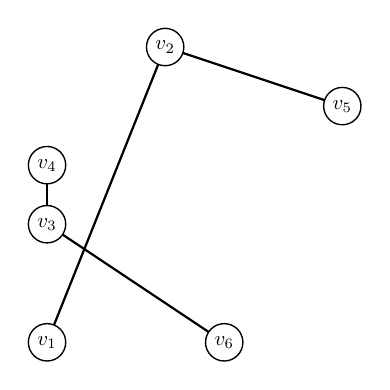
\begin{tikzpicture}[scale=0.75,transform shape]
\Vertex[x=0,y=0,L=$v_1$]{A}
\Vertex[x=2,y=5,L=$v_2$]{B}
\Vertex[x=0,y=2,L=$v_3$]{C}
\Vertex[x=0,y=3,L=$v_4$]{D}
\Vertex[x=5,y=4,L=$v_5$]{E}
\Vertex[x=3,y=0,L=$v_6$]{F}

\Edge(A)(B)
\Edge(C)(F)
\Edge(B)(E)
\Edge(C)(D)
\end{tikzpicture}

\end{center}
\end{figure}

\begin{definition}[Bipartiter Graph]
Wenn alle Knoten eines Graphen $G$ so in zwei disjunkte Mengen $S_1$ und $S_2$ (Partitionsklassen oder {\sl shores}) aufgeteilt werden können, dass keine Kanten von $G$ zwischen Knoten aus $S_1$ und solchen aus $S_2$ existieren, sprechen wir von einem bipartiten Graphen.
\end{definition}

Abbildung \ref{bipartGraph} illustriert einen bipartiten Graphen mit
\[
	V = S_1 \cup S_2 = \{v_1,v_2,v_5,v_7,v_8\} \cup \{ v_3,v_4,v_6,v_9 \}
\]
und
\[
	E = \left\{  \{v_1,v_3\}, \{v_2,v_3\}, \{v_2,v_9\}, \{v_4,v_8\}, \{v_5,v_6\}, \{ v_6,v_8 \}, \{ v_7,v_9 \}  \right\}.
\]

\begin{figure}
\caption{Ein bipartiter Graph}
\label{bipartGraph}
\begin{center}

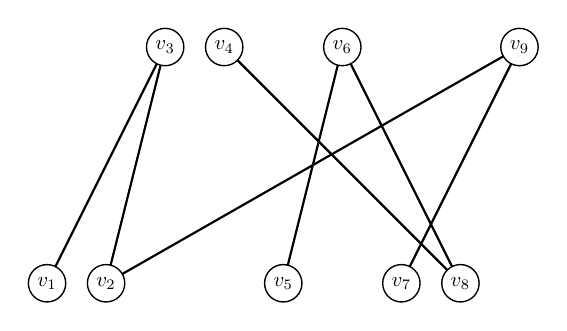
\begin{tikzpicture}[scale=0.75,transform shape]

\Vertex[x=0,y=0,L=$v_1$]{A1}
\Vertex[x=1,y=0,L=$v_2$]{A2}
\Vertex[x=2,y=4,L=$v_3$]{A3}
\Vertex[x=3,y=4,L=$v_4$]{A4}
\Vertex[x=4,y=0,L=$v_5$]{A5}
\Vertex[x=5,y=4,L=$v_6$]{A6}
\Vertex[x=6,y=0,L=$v_7$]{A7}
\Vertex[x=7,y=0,L=$v_8$]{A8}
\Vertex[x=8,y=4,L=$v_9$]{A9}

\Edge(A1)(A3)
\Edge(A2)(A3)
\Edge(A2)(A9)
\Edge(A7)(A9)
\Edge(A5)(A6)
\Edge(A6)(A8)
\Edge(A4)(A8)
\end{tikzpicture}

\end{center}
\end{figure}

\section{Zufallsgraphen}

Wenn wir Eigenschaften von vielen Graphen betrachten wollen, sind Zufallsgraphen ein hilfreicher Denkansatz. Das grundlegende Prinzip ist, eine feste Menge von Knoten $V$ anzunehmen und dann aus allen möglichen Kombinationen von Kanten (sprich aus der Potenzmenge $\mathcal{P}(E)$) mit einer definierten Wahrscheinlichkeit auszuwählen.

\bigskip
Das verbreitete Modell der Erdös-Renyi-Graphen definiert eine Klasse von Graphen $G(n, p)$ mit einer Anzahl Knoten $n$ und einer gleichverteilten Wahrscheinlichkeit $p$, dass eine Kante zwischen zwei Knoten besteht \cite{erdos}.

Da ein solcher Graph maximal $|\mathcal{P}(E)| = \binom{n}{2}$ Kanten haben kann, beträgt die Wahrscheinlichkeit, dass darin ein Graph mit genau $k$ Kanten auftritt, gegeben als
\[
\mathbb{P}(G) = p^k(1-p)^{\binom{n}{2}- k}.
\]

Es ist natürlich möglich, dass einzelne Knoten eines solchen Graphen gar keine Kanten haben, sprich das zusammenhängende Graph-Gebilde nicht alle $n$ Knoten beinhaltet. Diese Knoten werden aber trotzdem zum Graphen dazugezählt. \cite{erdos}

Abbildung \ref{pdistribution} zeigt die Auftretenswahrscheinlichkeit eines Graphen in $G(10, p)$ abhängig von der Anzahl Kanten für $p = 0.2, 0.5, 0.8.$

\begin{figure}
\caption{Verteilung der Auftretenswahrscheinlichkeit eines Zufallsgraphen}
\label{pdistribution}
\begin{center}
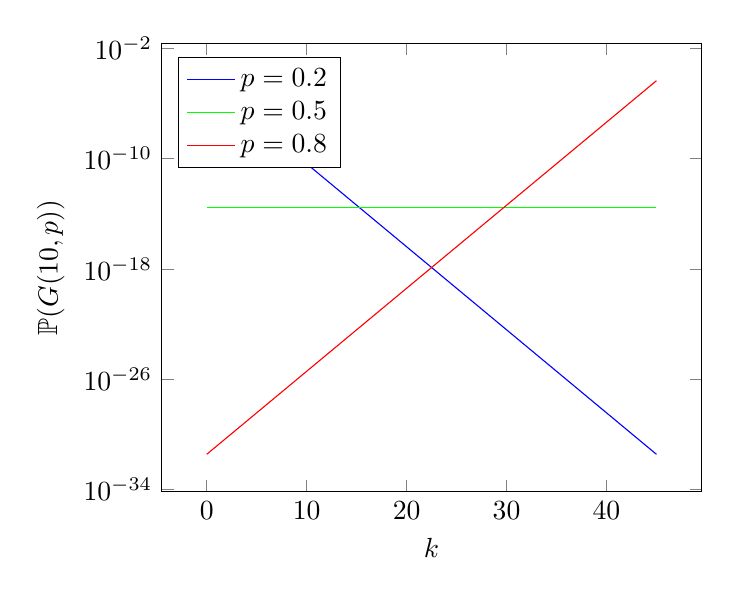
\begin{tikzpicture}
  \begin{semilogyaxis}[ 
    xlabel=$k$,
    ylabel={$\mathbb{P}(G(10, p))$},
	legend pos=north west
  ] 
    \addplot[mark=none,color=blue] coordinates {
(0,4.35561429658803E-05)
(1,1.08890357414701E-05)
(2,2.72225893536752E-06)
(3,6.8056473384188E-07)
(4,1.7014118346047E-07)
(5,4.25352958651175E-08)
(6,1.06338239662794E-08)
(7,2.65845599156984E-09)
(8,6.64613997892461E-10)
(9,1.66153499473115E-10)
(10,4.15383748682788E-11)
(11,1.03845937170697E-11)
(12,2.59614842926743E-12)
(13,6.49037107316857E-13)
(14,1.62259276829214E-13)
(15,4.05648192073035E-14)
(16,1.01412048018259E-14)
(17,2.53530120045647E-15)
(18,6.33825300114118E-16)
(19,1.58456325028529E-16)
(20,3.96140812571324E-17)
(21,9.90352031428309E-18)
(22,2.47588007857077E-18)
(23,6.18970019642693E-19)
(24,1.54742504910673E-19)
(25,3.86856262276683E-20)
(26,9.67140655691708E-21)
(27,2.41785163922927E-21)
(28,6.04462909807317E-22)
(29,1.51115727451829E-22)
(30,3.77789318629573E-23)
(31,9.44473296573934E-24)
(32,2.36118324143483E-24)
(33,5.90295810358708E-25)
(34,1.47573952589677E-25)
(35,3.68934881474193E-26)
(36,9.22337203685482E-27)
(37,2.30584300921371E-27)
(38,5.76460752303426E-28)
(39,1.44115188075857E-28)
(40,3.60287970189641E-29)
(41,9.00719925474104E-30)
(42,2.25179981368526E-30)
(43,5.62949953421315E-31)
(44,1.40737488355329E-31)
(45,3.51843720888322E-32)
	};
	\addlegendentry{$p = 0.2$}
    \addplot[mark=none,color=green] coordinates {
(0,2.8421709430404E-14)
(1,2.8421709430404E-14)
(2,2.8421709430404E-14)
(3,2.8421709430404E-14)
(4,2.8421709430404E-14)
(5,2.8421709430404E-14)
(6,2.8421709430404E-14)
(7,2.8421709430404E-14)
(8,2.8421709430404E-14)
(9,2.8421709430404E-14)
(10,2.8421709430404E-14)
(11,2.8421709430404E-14)
(12,2.8421709430404E-14)
(13,2.8421709430404E-14)
(14,2.8421709430404E-14)
(15,2.8421709430404E-14)
(16,2.8421709430404E-14)
(17,2.8421709430404E-14)
(18,2.8421709430404E-14)
(19,2.8421709430404E-14)
(20,2.8421709430404E-14)
(21,2.8421709430404E-14)
(22,2.8421709430404E-14)
(23,2.8421709430404E-14)
(24,2.8421709430404E-14)
(25,2.8421709430404E-14)
(26,2.8421709430404E-14)
(27,2.8421709430404E-14)
(28,2.8421709430404E-14)
(29,2.8421709430404E-14)
(30,2.8421709430404E-14)
(31,2.8421709430404E-14)
(32,2.8421709430404E-14)
(33,2.8421709430404E-14)
(34,2.8421709430404E-14)
(35,2.8421709430404E-14)
(36,2.8421709430404E-14)
(37,2.8421709430404E-14)
(38,2.8421709430404E-14)
(39,2.8421709430404E-14)
(40,2.8421709430404E-14)
(41,2.8421709430404E-14)
(42,2.8421709430404E-14)
(43,2.8421709430404E-14)
(44,2.8421709430404E-14)
(45,2.8421709430404E-14)
	};
	\addlegendentry{$p = 0.5$}
    \addplot[mark=none,color=red] coordinates {
(0,3.51843720888316E-32)
(1,1.40737488355326E-31)
(2,5.62949953421306E-31)
(3,2.25179981368522E-30)
(4,9.0071992547409E-30)
(5,3.60287970189636E-29)
(6,1.44115188075855E-28)
(7,5.76460752303418E-28)
(8,2.30584300921367E-27)
(9,9.2233720368547E-27)
(10,3.68934881474188E-26)
(11,1.47573952589675E-25)
(12,5.90295810358701E-25)
(13,2.36118324143481E-24)
(14,9.44473296573923E-24)
(15,3.77789318629569E-23)
(16,1.51115727451828E-22)
(17,6.04462909807311E-22)
(18,2.41785163922925E-21)
(19,9.67140655691699E-21)
(20,3.8685626227668E-20)
(21,1.54742504910672E-19)
(22,6.18970019642688E-19)
(23,2.47588007857075E-18)
(24,9.90352031428301E-18)
(25,3.96140812571321E-17)
(26,1.58456325028528E-16)
(27,6.33825300114113E-16)
(28,2.53530120045646E-15)
(29,1.01412048018258E-14)
(30,4.05648192073033E-14)
(31,1.62259276829213E-13)
(32,6.49037107316854E-13)
(33,2.59614842926741E-12)
(34,1.03845937170697E-11)
(35,4.15383748682787E-11)
(36,1.66153499473115E-10)
(37,6.64613997892459E-10)
(38,2.65845599156984E-09)
(39,1.06338239662794E-08)
(40,4.25352958651174E-08)
(41,1.7014118346047E-07)
(42,6.8056473384188E-07)
(43,2.72225893536752E-06)
(44,1.08890357414701E-05)
(45,4.35561429658803E-05)
	};
	\addlegendentry{$p = 0.8$}
  \end{semilogyaxis}
\end{tikzpicture}
\end{center}
\end{figure}

\floatname{algorithm}{Algorithmus}
\renewcommand{\algorithmicrequire}{\textbf{Eingabe:}}
\renewcommand{\algorithmicensure}{\textbf{Ausgabe:}}


\section{Generierung von Zufallsgraphen}

Zufallsgraphen zu generieren ist im Grunde genommen ziemlich einfach, wie Algorithmus~\ref{gen.naive} zeigt \cite{fastalgo}. Das Problem ist allerdings ebenfalls offensichtlich: Die Komplexitätsklasse dieses Algorithmus ist $\mathcal{O}(n^2)$.

\begin{algorithm}
\caption{Ein naiver Zufallsgraphen-Generator}
\label{gen.naive}
\begin{algorithmic}
\Require
	\Statex Anzahl Knoten $n$,
	\Statex Kantenwahrscheinlichkeit $p$.
\Ensure
	\Statex Zufallsgraph $G = (V, E)$.
\Statex
\For{$i \gets 1, n$}
\For{$j \gets i+1, n$}
\State $\theta\gets$ gleichverteilte Zufallszahl
\If{$\theta < p$}
\State $E \gets E \cup \{(v_i,v_j)\}$
\EndIf
\EndFor
\EndFor
\end{algorithmic}
\end{algorithm}


Um diese technische Suboptimalität zu lösen, verfolgen Nobari, Lu, Karras und Bressan in \cite{fastalgo} folgende Idee:

\begin{enumerate}
\item Jede Kante $(v_i, v_j)$ (und darum auch $\{v_i, v_j\}$) kann als $e_k$ ausgedrückt werden durch die Beziehungen
\[
i = \left\lfloor\frac k v \right\rfloor
\]
und
\[
j = k \mod v.
\]

\item Damit kann Algorithmus~\ref{gen.naive} $\in \mathcal{O}(n^2)$ zu einem Algorithmus mit linearer Laufzeitkomplexität $\mathcal{O}(|E|)$ umgeschrieben werden (siehe Algorithmus~\ref{gen.linear}). Da aber $|E| = \binom{n}{2}$ gilt, nützt uns das momentan noch nicht viel.

\begin{algorithm}
\caption{Ein umgeformter naiver Zufallsgraphen-Generator}
\label{gen.linear}
\begin{algorithmic}
\Require
	\Statex Kantenwahrscheinlichkeit $p$.
\Ensure
	\Statex Zufallsgraph $G = (V, E)$.
\Statex
\For{$i \gets 1, |E|$}
\State $\theta\gets$ gleichverteilte Zufallszahl
\If{$\theta < p$}
\State $E \gets E \cup \{e_i\}$
\EndIf
\EndFor
\end{algorithmic}
\end{algorithm}

\item Der eigentliche Trick folgt der Erkenntnis, dass die Wahrscheinlichkeitsverteilung einer Folge von gleichverteilten Zufallsentscheidungen, die zum selben Resultat führen, im Grunde einer geometrischen Verteilung entspricht. Dadurch können wir die Wahrscheinlichkeit, dass die nächsten $s$ Kanten des Graphen mit einer jeweiligen Wahrscheinlichkeit von $1-p$ ausgelassen werden, ausdrücken als
\[
	f(s) = p \cdot (1-p)^s,
\]
und die kumulative Verteilungsfunktion wäre (\cite{fastalgo})
\[
	F(s) = \sum\limits_{i=0}^s f(i) = 1 - (1-p)^{s+1}.
\]
Dies bedeutet, dass der Algorithmus nach jedem Setzen einer Kante eine einzige neue Zufallszahl $\alpha$ generiert, mit welcher er bestimmen kann, wieviele Kanten $s$ ausgelassen werden können (nämlich die kleinste ganze Zahl, für welche
\[
F(s) \ge \alpha
\]
gilt). Durch ein paar Takte Algebra können wir nach $s$ auflösen und bekommen eine explizite Funktion (\cite{fastalgo}):
\[
	s(\alpha) = \max(0, \left\lceil \log_{1-p}\alpha\right\rceil - 1)
\]

Damit können wir unseren Algorithmus optimieren (siehe Algorithmus~\ref{gen.opt}). Es liegt nun auf der Hand, dass dieser Algorithmus desto schneller ist, je kleiner $p$ gewählt wird. \cite{fastalgo} versucht darum, der durch die Berechnung des Logarithmus gestiegenen mathematischen Komplexität Herr zu werden, indem eine Menge an Logarithmus-Werten vorberechnet und wiederverwendet werden. Ausserdem werden noch Optimierungen vorgenommen, um den Algorithmus auf Grafik-Prozessoren laufen zu lassen. Dies ist für uns allerdings nicht weiter spannend, und darum wollen wir es bei der einfachen Optimierung wie eben gesehen belassen.

\begin{algorithm}
\caption{Ein Zufallsgraphen-Generator mit Edge Skipping}
\label{gen.opt}
\begin{algorithmic}
\Require
	\Statex Kantenwahrscheinlichkeit $p$.
\Ensure
	\Statex Zufallsgraph $G = (V, E)$.
\Statex
\Statex $i \gets -1$
\While{$i < |E|$}
\State $\alpha\gets$ gleichverteilte Zufallszahl
\State $s \gets \max(0, \left\lceil \log_{1-p}\alpha\right\rceil - 1)$
\State $i \gets i + s + 1$
\State $E \gets E \cup \{e_i\}$
\EndWhile
\State Entferne die letzte Kante
\end{algorithmic}
\end{algorithm}

\end{enumerate}

\section{Generierung von bipartiten Zufallsgraphen}



\bibliography{biblio}
\bibliographystyle{plain}




\end{document}
